\documentclass[a4paper,11pt,titlepage]{scrbook}
\usepackage[utf8]{inputenc}
\usepackage[spanish]{babel}

% \usepackage[style=list, number=none]{glossary} %si se va a usar glosario, quitar marca de comentario
%\usepackage{titlesec}
%\usepackage{palatino} %usar fot palatino en vez de times roman

%\decimalpoint %revisar
%\usepackage{dcolumn} %revisat
%\newcolumntype{.}{D{.}{\esperiod}{-1}}
%\makeatletter
%\addto\shorthandsspanish{\let\esperiod\es@period@code}
%\makeatother


%\usepackage[chapter]{algorithm}
%\RequirePackage{verbatim}
%\RequirePackage[Glenn]{fncychap}
\usepackage{fancyhdr}
\usepackage{graphicx}
\usepackage{afterpage}
\usepackage{longtable}
\usepackage{xcolor}
\definecolor{portada}{RGB}{239,206,53}
\definecolor{base}{RGB}{35,31,32}
\usepackage{pdfpages}


%Instrucciones para poder escribir código y mostrarlo de manera elegante:
\definecolor{gray97}{gray}{.97}
\definecolor{gray75}{gray}{.75}
\definecolor{gray45}{gray}{.45}
\definecolor{gray30}{gray}{.94}

\usepackage{listings}
\lstset{ frame=Ltb,
framerule=0pt,
aboveskip=0.5cm,
framextopmargin=3pt,
framexbottommargin=3pt,
framexleftmargin=0.4cm,
framesep=0pt,
rulesep=.4pt,
backgroundcolor=\color{gray97},
rulesepcolor=\color{black},
%
stringstyle=\ttfamily,
showstringspaces = false,
basicstyle=\small\ttfamily,
commentstyle=\color{gray45},
keywordstyle=\bfseries,
%
numbers=left,
numbersep=15pt,
numberstyle=\tiny,
numberfirstline = false,
breaklines=true,
literate={á}{{\'a}}1 {Á}{{\'A}}1 {é}{{\'e}}1 {É}{{\'e}}1 {í}{{\'i}}1  {Í}{{\'I}}1  {ó}{{\'o}}1  {Ó}{{\'O}}1  {ú}{{\'u}}1  {Ú}{{\'U}}1  {Ñ}{{\~N}}1 {ñ}{{\~n}}1 ,
}



% minimizar fragmentado de listados
\lstnewenvironment{listing}[1][]
   {\lstset{#1}\pagebreak[0]}{\pagebreak[0]}

\lstdefinestyle{Consola}
   {basicstyle=\scriptsize\bf\ttfamily,
    backgroundcolor=\color{gray30},
    frame=single,
    numbers=none
   }
\lstdefinestyle{C}
	{basicstyle=\scriptsize,
	frame=single,
	language=C,
	numbers=left
	}
\lstdefinestyle{CodigoC++}
        {basicstyle=\small,
	frame=single,
	backgroundcolor=\color{gray30},
	language=C++,
	numbers=left
 	}
\lstdefinestyle{PHP}
	{basicstyle=\scriptsize,
%        {basicstyle=\small,
	frame=single,
	language=PHP,
	numbers=left
	}
	



% ********************************************************************
% Información sobre el TFG. Comentar lo que NO se desee añadir y sustituir con la información correcta.
% ********************************************************************
\newcommand{\myTitle}{Título del Trabajo de Fin de Grado}
\newcommand{\mySubtitle}{Subtítulo del proyecto}
\newcommand{\myDegree}{Grado en Ingeniería Multimedia}
\newcommand{\myName}{Nombre Apellido1 Apellido2 (alumno)}
\newcommand{\myProf}{Nombre Apellido1 Apellido2 (tutor1)}
\newcommand{\myOtherProf}{Nombre Apellido1 Apellido2 (tutor2)}
\newcommand{\myFaculty}{Escuela Politécnica Superior de la Universidad de Alicante}
\newcommand{\myFacultyShort}{EPS UA}
\newcommand{\depTutorOne}{Departamento del tutor}
\newcommand{\depTutorTwo}{Departamento del cotutor}


\newcommand{\myUni}{\protect{Universidad de Alicante}}
\newcommand{\myLocation}{Alicante}
\newcommand{\myTime}{\today}
%\newcommand{\myVersion}{Version 0.1}

\newcommand{\logoGrado}{imagenes/logoim.jpg}
\newcommand{\logoFacultad}{imagenes/logoeps.jpg}
\newcommand{\logoUniversidad}{imagenes/logoua.jpg}

\usepackage{url}

% Definición de comandos que me son útiles:
%\renewcommand{\indexname}{Índice alfabético}
%\renewcommand{\glossaryname}{Glosario}

\pagestyle{fancy}
\fancyhf{}
\fancyhead[LO]{\leftmark}
\fancyhead[RE]{\rightmark}
\fancyhead[RO,LE]{\textbf{\thepage}}
\renewcommand{\chaptermark}[1]{\markboth{\textbf{#1}}{}}
\renewcommand{\sectionmark}[1]{\markright{\textbf{\thesection. #1}}}


\setlength{\headheight}{1.5\headheight}

\newcommand{\HRule}{\rule{\linewidth}{0.5mm}}
%Definimos los tipos teorema, ejemplo y definición podremos usar estos tipos
%simplemente poniendo \begin{teorema} \end{teorema} ...
\newtheorem{teorema}{Teorema}[chapter]
\newtheorem{ejemplo}{Ejemplo}[chapter]
\newtheorem{definicion}{Definición}[chapter]
 
\newcommand{\bigrule}{\titlerule[0.5mm]}


%Para conseguir que en las páginas en blanco no ponga cabeceras
\makeatletter
\def\clearpage{%
  \ifvmode
    \ifnum \@dbltopnum =\m@ne
      \ifdim \pagetotal <\topskip
        \hbox{}
      \fi
    \fi
  \fi
  \newpage
  \thispagestyle{empty}
  \write\m@ne{}
  \vbox{}
  \penalty -\@Mi
}
\makeatother

\usepackage[pdfborder={000}]{hyperref} %referencia
\hypersetup{
pdfauthor = {\myName (email (en) ua (punto) es)},
pdftitle = {\myTitle},
pdfsubject = {},
pdfkeywords = {palabra_clave1, palabra_clave2, palabra_clave3, ...},
pdfcreator = {LaTeX con el paquete ....},
pdfproducer = {pdflatex}
}
%AQUI COMIENZA LA LISTA DE FICHEROS A INCLUIR



\begin{document}
\renewcommand{\listtablename}{Índice de tablas} %para sustituir la palabra cuadro por tabla
\renewcommand{\tablename}{Tabla}
\renewcommand{\lstlistingname}{Listado}
\renewcommand{\lstlistlistingname}{Índice de \lstlistingname s}

\frontmatter
\begin{titlepage}

\newlength{\centeroffset}
\setlength{\centeroffset}{-0.5\oddsidemargin}
\addtolength{\centeroffset}{0.5\evensidemargin}
\thispagestyle{empty}

\includepdf[pages={1},pagecommand={},fitpaper=true,trim=0 0 0 0, 
offset=0 0,turn=true,noautoscale=true]{portada/portada.pdf}

\end{titlepage}
\pagecolor{white} %la portada en color
\begin{titlepage}
 
 
\setlength{\centeroffset}{-0.5\oddsidemargin}
\addtolength{\centeroffset}{0.5\evensidemargin}
\thispagestyle{empty}

\noindent\hspace*{\centeroffset}\begin{minipage}{\textwidth}

\centering


% Title

%{\Huge\bfseries Título del proyecto\\ }
{\Huge\bfseries \myTitle}

\noindent\rule[-1ex]{\textwidth}{3pt}\\[3.5ex]
{\large\bfseries \mySubtitle\\[4cm]}
\end{minipage}

\vspace{2.5cm}
\noindent\hspace*{\centeroffset}\begin{minipage}{\textwidth}
\centering

\textbf{Autor}\\ {\myName}\\[2.5ex]
\textbf{Directores}\\
{\normalsize \myProf\\
\small\textit \depTutorOne\\
\normalsize \myOtherProf\\
\small\textit \depTutorTwo\\[2cm]}

\includegraphics[scale=0.25]{\logoGrado}


\textsc{\myDegree}\\

\centering
\begin{minipage}[l]{7cm}
\includegraphics[width=5cm]{\logoFacultad}
\end{minipage}
\begin{minipage}[r]{7cm}
\includegraphics[width=5cm]{\logoUniversidad}
\end{minipage}


%\textsc{\myFaculty}\\

%\large\bfseries \textsc{\myUni}\\
ALICANTE, \myTime

\end{minipage}
%\addtolength{\textwidth}{\centeroffset}
\vspace{\stretch{2}}

\end{titlepage}


 %la portada en b/n
\chapter*{Preámbulo}
\thispagestyle{empty}
Poner aquí un texto breve que debe incluir entre otras:
\begin{quote}
``las razones que han llevado a la realización del estudio, el tema, la finalidad y el alcance y también los agradecimientos por las ayudas, por ejemplo apoyo económico (becas y subvenciones) y las consultas y discusiones con los tutores y colegas de trabajo. \cite{UNE50136:97}''
\end{quote}

\cleardoublepage %salta a nueva página impar
% Aquí va la dedicatoria si la hubiese. Si no, comentar la(s) linea(s) siguientes
\chapter*{}
\setlength{\leftmargin}{0.5\textwidth}
\setlength{\parsep}{0cm}
\addtolength{\topsep}{0.5cm}
\begin{flushright}
\small\em{
A mi esposa Marganit, y a mis hijos Ella Rose y Daniel Adams,\\
sin los cuales habría podido acabar este libro dos años antes \footnote{Dedicatoria de Joseph J. Roman en ``An Introduction to Algebraic Topology''}
}
\end{flushright}


\cleardoublepage %salta a nueva página impar
% Aquí va la cita célebre si la hubiese. Si no, comentar la(s) linea(s) siguientes
\chapter*{}
\setlength{\leftmargin}{0.5\textwidth}
\setlength{\parsep}{0cm}
\addtolength{\topsep}{0.5cm}
\begin{flushright}
\small\em{
Si consigo ver más lejos\\
es porque he conseguido auparme\\ 
a hombros de gigantes
}
\end{flushright}
\begin{flushright}
\small{
Isaac Newton.
}
\end{flushright}
\cleardoublepage %salta a nueva página impar
 %editar este texto (capitulos/preliminares.tex) para cambiar preámbulo, agradecimientos y dedicatorias
\tableofcontents
\listoffigures
\listoftables
\lstlistoflistings

\mainmatter %entre frontmatter y mainmatter, la numeración es en romanos.

%a continuación se propone un esquema de trabajo que puede ser alterado justificadamente.
\chapter{Introducción}
\section{¡Importante!, leer primero}

Este texto está escrito pensando en orientar a los alumnos que usarán \LaTeX para escribir sus TFG de Ingeniería Multimedia.

Contiene información útil para aquellos que no tengan experiencia previa en \LaTeX así como algunos datos acerca de cómo escribir mejor su TFG.

A continuación, se ofrece una copia de la información que hay en el libro de estilo para la realización de los TFG de la EPS de la Universidad de Alicante.

En el siguiente capítulo (página \pageref{marcoteorico}) encontrarás algunos ejemplos de cómo hacer listas, tablas y otras estructuras de un texto en \LaTeX. Con un poco de paciencia, estudia cómo se hacen estas cosas y luego aplícalas en tus documentos.

\section{Estructura de un TFG}

En caso de que el TFG/TFM tenga como finalidad la elaboración de un proyecto o un 
informe científico o técnico, deberá ajustarse a lo dispuesto en las normas UNE 
157001:2002 y UNE 50135:1996 respectivamente.

Si el TFG/TFM tiene por finalidad la elaboración de un trabajo monográfico, el 
documento presentado deberá constar de las siguientes partes, teniendo como base la 
norma UNE 50136:1997.

\begin{description}
\item[Preámbulo:] se describirán brevemente la motivación que ha originado la realización del TFG/TFM, así como de una breve descripción de los objetivos generales que se quieren alcanzar con el trabajo presentado.
\item[Agradecimientos:] se podrá añadir las hojas necesarias para realizar los agradecimientos, a veces obligatorios, a las entidades y organismos colaboradores.
\item[Dedicatoria:] se podrá añadir una única hoja con dedicatorias, su alineación será derecha y centradas de forma distribuida en la página.
\item[Citas:] (frases célebres) se podrá añadir una única hoja con citas, su alineación será derecha y centradas de forma distribuida en la página.
\item[Índices:] cada índice debe comenzar en una nueva página, se incluirán los índices que se estimen necesarios (conforme UNE 50111:1989), en este orden:
\begin{description}
\item[Índice de contenidos:] (obligatorio siempre) se incluirá un índice de las secciones de las que se componga el documento, la numeración de las 
divisiones y subdivisiones utilizarán cifras arábigas (según UNE 50132:1994) y harán mención a la página del documento donde se ubiquen.
\item[Índice de figuras:] si el documento incluye figuras se podrá incluir también un índice con su relación, indicando la página donde se ubiquen.
\item[Índice de tablas:] en caso de existir en el texto, ídem que el anterior.
\item[Índice de abreviaturas, siglas, símbolos, etc.:] en caso de ser necesarios se podrá incluir cada uno de ellos.
\end{description}
\item[Cuerpo del documento:] en el contenido del documento se da flexibilidad para su organización y se puede estructurar en las secciones que se considere. En todo caso obligatoriamente se deberá, al menos, incluir los siguientes contenidos:
\begin{description}
\item[Introducción:] donde se hará énfasis a la importancia de la temática, su vigencia y actualidad; se planteará el problema a investigar, así como el propósito o finalidad de la investigación.
\item[Marco teórico o Estado del arte:] se hará mención a los elementos conceptuales que sirven de base para la investigación, estudios previos relacionados con el problema planteado, etc.
\item[Objetivos:] se establecerá el objetivo general y los específicos.
\item[Metodología:] se indicará el tipo o tipos de investigación, las técnicas y los procedimientos que serán utilizados para llevarla a cabo; se identificará la población y el tamaño de la muestra así como las técnicas e instrumentos de recolección de datos.
\item[Resultados:] incluirá los resultados de la investigación o trabajo, así como el análisis y la discusión de los mismos.
\end{description}
\item[Conclusiones:] obligatoriamente se incluirá una sección de conclusiones donde se realizará un resumen de los objetivos conseguidos así como de los resultados obtenidos si proceden.
\item[Bibliografía y referencias:] se incluirá también la relación de obras y materiales consultados y empleados en la elaboración de la memoria del TFG/TFM. La bibliografía y las referencias serán indexadas en orden alfabético (sistema nombre y fecha) o se numerará correlativamente según aparezca (sistema numérico). Se empleará la familia 1 como tipo de letra. Podrá utilizarse cualquier sistema bibliográfico normalizado predominante en la rama de conocimiento, estableciéndose como prioritarios el sistema ISO 690, sistema APA (American Psychological Association) o Harvard (no necesariamente en ese orden de preferencia). En esta plantilla Latex se propone usar el estilo APA indicándolo en la línea correspondiente como 
\begin{verbatim}
\bibliographystyle{apalike}
\end{verbatim}


\item[Anexos:] se podrá incluir los anexos que se consideren oportunos.

\end{description}




\chapter{Marco Teórico}
\label{marcoteorico}

El contenido de este capítulo es una especie de muestrario de cosas que puedes hacer con \LaTeX.  Por ejemplo, incluir una cita bibliográfica   \cite{BOE_IM_UA} dentro del texto. En esta página de demostración también puedes encontrar información útil acerca de cómo escribir con  \LaTeX.\footnote{En http://metodos.fam.cie.uva.es/~latex/apuntes/apuntes.html hay unos buenos apuntes al respecto.}

Hacer una lista es simple en \LaTeX. Para ello has de crear un entorno (así se llama) itemize con
\begin{verbatim}
\begin{itemize}
...
\end{itemize}
\end{verbatim}
Y dentro de esa estructura, añadir cada elemento de la lista precedido de 
\begin{verbatim}
\item primer item de lista
\item segundo item de lista
...
\item ultimo item de lista
\end{verbatim}
\section{Elaboración de listas.}

Es importante que revises este texto tal como aparece en la plantilla y relaciones el aspecto que tiene el PDF final con cómo está escrito el documento \LaTeX.

Aquí va una lista:
\begin{itemize}
    \item Ingeniería Informática.
    \item Ingeniería Sonido e Imagen en Telecomunicación.
    \item Ingeniería Multimedia.
    \begin{itemize}
         \item Mención: Creación y ocio digital.
         \item Mención: Gestión de Contenidos.
    \end{itemize}
\end{itemize}

Ahora veremos otra estructura más: las tablas.

\section{Inserción de tablas}

Aquí va una tabla\footnote{En http://www.tablesgenerator.com/ se puede encontrar un generador On-Line de tablas para \LaTeX} para que se vea cómo insertar una tabla simple dentro del documento.

\begin{table}[h]
\begin{center}
\begin{tabular}{lllll}
&columna A&columna B&columna C\\
\hline
fila 1&fila 1, columna A & fila 1, columna B & fila 1, columna C\\
fila 2&fila 2, columna A & fila 2, columna B & fila 2, columna C\\
fila 3&fila 3, columna A & fila 3, columna B & fila 3, columna C\\ \hline
\end{tabular}
\end{center}
\caption{Ejemplo de tabla.}
\label{tabladeejemplo}
\end{table}

\LaTeX usa un sistema de parámetros para ``decorar'' las tablas. Puedes consultar estos parámetros en la tabla \ref{tabla_parametros} de la página \pageref{tabla_parametros}. La tabla se ubicará donde, a juicio de \LaTeX, menos moleste por lo que puede no aparecer necesariamente donde se ha insertado en el texto original. 

\begin{table}
\begin{center}
\begin{tabular}{|c|p{0.8\textwidth}|}
\hline
Parámetro & \multicolumn{1}{c|}{Significado} \\ \hline
\texttt{h} & Situa el elemento flotante \emph{preferentemente}
(es decir, si es posible) en la situación exacta donde se incluye este \\
\texttt{t} & Situa el elemento en la parte de arriba de la página \\
\texttt{b} & Situa el elemento en la parte de abajo de la página \\
\texttt{p} & Situa el elemento en una página aparte dedicada sólo a
elementos flotantes; en el caso del formato \texttt{article},
ésta se situa al final del documento, mientras que para al book es
colocada al final de cada capítulo \\ \hline
\end{tabular}
\end{center}
\caption{Parámetros optativos de los entornos flotantes}
\label{tabla_parametros}
\end{table}



\section{Inserción de figuras}

Las figuras son un caso un poco especial ya que \LaTeX busca el mejor lugar para ponerlas, no siendo necesariamente el ligar donde está la referencia. Por ello es importante añadirle un ``caption'' y un ``label'' para poder hacer referencia a ellas en el párrafo correspondiente. Nosotros ponemos la referencia a la figura \ref{logo_im} que está en la página \pageref{logo_im}. justo aquí debajo, pero \LaTeX puede que la ubique en otro lugar.

\begin{figure}
\begin{center}
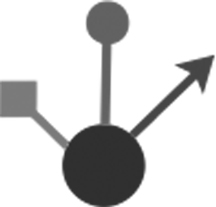
\includegraphics[scale=0.25]{imagenes/logoim.jpg}
\caption{Logo de Ingeniería  Multimedia.}
\label{logo_im}
\end{center}
\end{figure}

\begin{figure}
\begin{center}

\includegraphics[scale=0.25]{imagenes/logoeps.jpg}
\caption{Logo de la EPS.}
\label{logo_eps}
\end{center}
\end{figure}

\section{Inserción de código}
A veces tendrás que insertar algún pedazo de código fuente para explicar algo relacionado con él. No sustituyas explicaciones con enormes listados de código. Si pones algo de código en tu TFG que sea para demostrar algo o explicar alguna solución.

\LaTeX te ayuda a escribir código de manera que su presentación tenga las marcas y tabulaciones propias de este tipo de texto. Para ello, debes poner el código que escribas DENTRO de un entorno  que se llama ``listings''.  La plantilla ya tiene una serie de instrucciones para incluir el paquete ``listings'' y añadirle algunos modificadores por lo que no tienes que incluirlo tú. Simplemente, mete tu código en el entorno ``lstlisting'' y ya está. Puedes indicar el lenguaje en el que está escrito el código y así \LaTeX lo mostrará mejor. Veamos un ejemplo en la figura \ref{C_code}:

Si pones 
\begin{verbatim}
\begin{lstlisting}[style=C, caption={ejemplo código C},label=C_code]
#include <stdio.h>
int main(int argc, char* argv[]) {
  puts("Hola mundo!");
}
\end{lstlisting}
\end{verbatim}

El resultado será:
\begin{lstlisting}[style=C, caption={ejemplo código C},label=C_code]
#include <stdio.h>
int main(int argc, char* argv[]) {
  puts("Hola mundo!");
}
\end{lstlisting}

Por supuesto, puedes mejorar esta presentación utilizando mas modificadores. Esta información y mucha más puede ser encontrada en \cite{listing_packagge} y en \cite{heinz1listings}.

Otro ejemplo, ahora para mostrar código PHP, sería escribir en tu fichero \LaTeX lo siguiente:
\begin{verbatim}
 \begin{lstlisting}[style=PHP, caption={ejemplo código PHP},label=PHP_code]
 /* 
Ejemplo de código en PHP para escribir tu primer programa en este lenguaje
Copia este código en tu ordenador y ejecútalo
*/
<html>
  <head>
    <title>Prueba de PHP</title>
  </head>
  <body>
    <?php echo '<p>Hola Mundo</p>'; ?> //esto lo escribe TODO el mundo
  </body>
</html>
 \end{lstlisting}
\end{verbatim}
 
 y el resultado es: (ver listado \ref{PHP_code})
 
 \begin{lstlisting}[style=PHP, caption={ejemplo código PHP},label=PHP_code]
/* 
Ejemplo de código en PHP para escribir tu primer programa en este lenguaje. Copia este código en tu ordenador y ejecútalo
*/
 <html>
  <head>
    <title>Prueba de PHP</title>
  </head>
  <body>
    <?php echo '<p>Hola Mundo</p>'; ?> //esto lo escribe TODO el mundo
  </body>
</html>
 \end{lstlisting}
 
 Observa cómo \LaTeX ha puesto los comentarios en gris y ajustado el código para que se muestre más claro.
 
 Si quieres añadir código en otros lenguajes, cambia el comando que dice ``style=nombredellenguaje'' por ``languaje=nombredelnuevolenguaje''.
%input{capitulos/objetivos}
%input{capitulos/metodologia}
%input{capitulos/desarrollo}
%input{capitulos/resultados}
%input{capitulos/conclusiones}

%%\nocite{*} %incluye TODOS los documentos de la base de datos bibliográfica sean o no citados en el texto
\bibliography{bibliografia/bibliografia}\addcontentsline{toc}{chapter}{Bibliografía} %sustituir bibliografía con el nombre del fichero bibtex con la bibliografía
\bibliographystyle{apalike}
%
\appendix
\chapter{Anexo I}
Aquí vendría en anexo I 
%\input{glosario/entradas_glosario}
% \addcontentsline{toc}{chapter}{Glosario} %si se usa glosario hay que añadirlo al índice
% \printglossary %muestra el glosario

\end{document}
